\chapter{La combustion~: combustibles, produits et gaz à effet de serre}\label{ch:g8:combustion-and-fuels}

Une famille dort dans un appartement dont la chaudière à gaz a un conduit
d'évacuation bouché. La flamme, privée d'\omterm{def:g4:air-a-mixture-of-gases:air}{air}, \omterm{def:g4:what-a-fire-needs:burning}{brûle} mal, et un gaz
invisible et sans odeur envahit lentement les pièces. À deux heures du
matin, un petit boîtier fixé au mur se met à hurler~: le détecteur de
monoxyde de carbone. Tout le monde sort à temps. Le même \omterm{def:g4:what-a-fire-needs:fuel}{combustible},
quand il \omterm{def:g4:what-a-fire-needs:burning}{brûle} bien, ne donne que du dioxyde de carbone et de l'eau ---
et ce dioxyde de carbone a sa propre histoire, inscrite dans l'\omterm{def:g4:air-a-mixture-of-gases:air}{air} de la
planète entière.

\begin{recall}
Une \omterm{def:g4:what-a-fire-needs:burning}{combustion} a besoin d'un \omterm{def:g4:what-a-fire-needs:fuel}{combustible}, de dioxygène et de chaleur, et
fabrique de nouvelles substances (\cref{ch:g4:what-a-fire-needs}). L'\omterm{def:g4:air-a-mixture-of-gases:air}{air}
contient environ un cinquième de dioxygène
(\cref{ch:g4:air-a-mixture-of-gases}). Une équation est ajustée quand
chaque sorte d'\omterm{def:g7:atoms-and-molecules:atom}{atome} apparaît le même nombre de fois des deux côtés
(\cref{ch:g8:balanced-equations}).
\end{recall}

\section{La combustion du carbone et du méthane}

\begin{example}[Deux combustions]\label{ex:g8:combustion-and-fuels:two}
Le carbone (charbon de bois, houille) \omterm{def:g4:what-a-fire-needs:burning}{brûle} en donnant du dioxyde de
carbone~:
\[
  \ce{C(s) + O2(g) -> CO2(g)}.
\]
Le méthane, principal constituant du gaz naturel, \omterm{def:g4:what-a-fire-needs:burning}{brûle} en donnant du
dioxyde de carbone et de l'eau~:
\[
  \ce{CH4(g) + 2O2(g) -> CO2(g) + 2H2O(l)}.
\]
Dans les deux cas, l'eau de chaux se trouble avec le gaz formé~; avec
le méthane, un verre froid se couvre aussi de buée.
\end{example}

\begin{method}[Écrire la combustion d'un combustible fait de carbone et d'hydrogène]\label{met:g8:combustion-and-fuels:write}
Pour un \omterm{def:g4:what-a-fire-needs:fuel}{combustible} dont les \omterm{def:g7:atoms-and-molecules:molecule}{molécules} ne contiennent que du carbone et
de l'hydrogène~:
\begin{enumerate}
  \item les produits sont le dioxyde de carbone et l'eau~;
  \item ajuster le carbone avec \ce{CO2}, puis l'hydrogène avec
        \ce{H2O}~;
  \item compter les \omterm{def:g7:atoms-and-molecules:atom}{atomes} d'oxygène à droite et les ajuster avec
        \ce{O2}~; tout doubler si une moitié apparaît.
\end{enumerate}
Pour le butane~: \ce{2C4H10 + 13O2 -> 8CO2 + 10H2O}.
\end{method}

\section{Combustion complète et combustion incomplète}

\begin{definition}[Combustion complète et combustion incomplète]\label{def:g8:combustion-and-fuels:complete}
Une \emph{combustion complète}\index{combustion complete@combustion complète} a lieu avec
assez de dioxygène~: tout le carbone du \omterm{def:g4:what-a-fire-needs:fuel}{combustible} devient du dioxyde
de carbone. Une \emph{combustion incomplète}\index{combustion incomplete@combustion incomplète}
a lieu avec trop peu de dioxygène~: une partie du carbone devient du
monoxyde de carbone, \ce{CO}, ou de la suie, qui est du carbone, \ce{C}.
\end{definition}

\begin{example}[Le méthane à court de dioxygène]\label{ex:g8:combustion-and-fuels:incomplete}
Avec trop peu d'\omterm{def:g4:air-a-mixture-of-gases:air}{air}, le méthane peut \omterm{def:g4:what-a-fire-needs:burning}{brûler} en donnant du monoxyde de
carbone ou de la suie~:
\[
  \ce{2CH4 + 3O2 -> 2CO + 4H2O}, \qquad \ce{CH4 + O2 -> C + 2H2O}.
\]
\end{example}

\begin{proposition}[Lire une flamme]\label{prop:g8:combustion-and-fuels:flame}
Un bec Bunsen dont la virole est ouverte \omterm{def:g6:pure-substances-and-mixtures:mixture}{mélange} de l'\omterm{def:g4:air-a-mixture-of-gases:air}{air} au gaz avant
qu'il \omterm{def:g4:what-a-fire-needs:burning}{brûle}~: la flamme est bleue et à peine visible, la \omterm{def:g8:combustion-and-fuels:complete}{combustion
complète}. Virole fermée, le gaz trouve trop peu de dioxygène~: la flamme
est jaune, fumeuse, et noircit de suie un objet froid qu'on y tient ---
la \omterm{def:g4:what-a-fire-needs:burning}{combustion} est incomplète.
\end{proposition}

\begin{omfigure}
\begin{tikzpicture}[font=\small, scale=1.3]
  \pic[transform shape] at (0,0) {bunsen=open};
  \node[anchor=north, align=center] at (0,-0.1) {virole ouverte~:\\ flamme bleue, complète};
  \pic[transform shape] at (4,0) {bunsen=closed};
  \node[anchor=north, align=center] at (4,-0.1) {virole fermée~:\\ flamme jaune, incomplète};
  \draw[<-, omProp, thick] (0.08,0.6) -- (1.4,0.9) node[right, text=black] {arrivée d'air};
  \draw[<-, omProp, thick] (-0.4,0.3) -- (-1.3,0.6) node[left, text=black] {gaz};
  \draw[<-, omProp, thick] (4.15,3.3) -- (5.0,3.5) node[right, text=black, align=left]
    {suie, monoxyde\\ de carbone};
\end{tikzpicture}

{\small Un bec Bunsen. De l'\omterm{def:g4:air-a-mixture-of-gases:air}{air} admis à la base donne une flamme bleue et
une \omterm{def:g8:combustion-and-fuels:complete}{combustion complète}~; sans lui, la flamme est jaune et fumeuse.}
\end{omfigure}

\begin{omfigure}
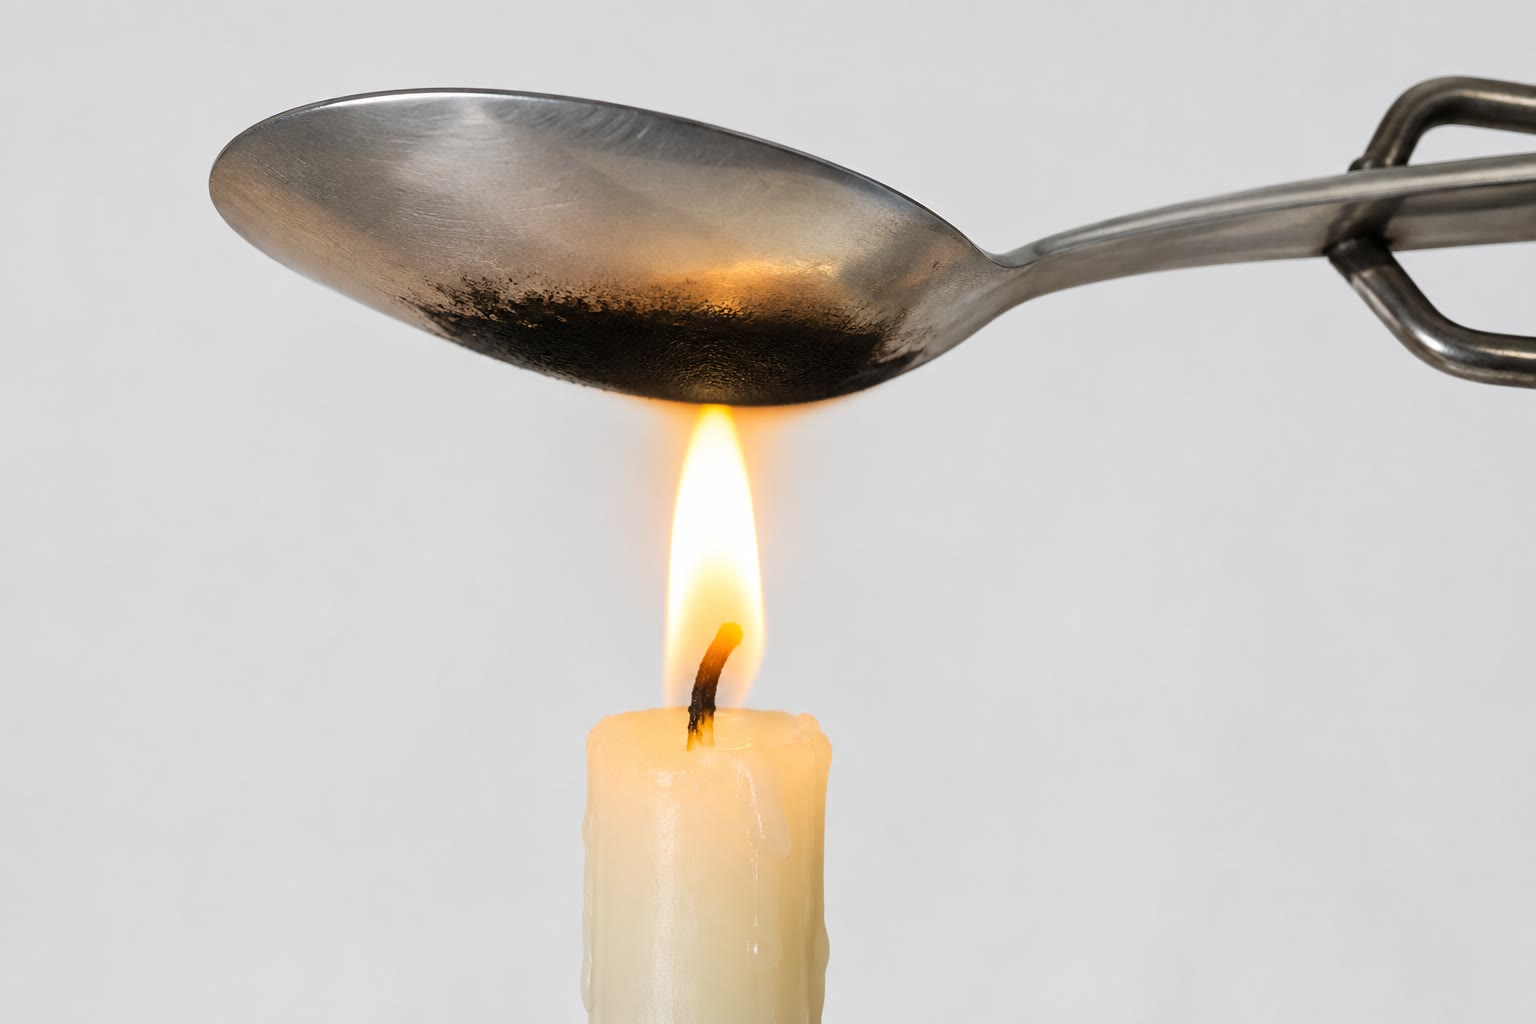
\includegraphics[width=0.45\linewidth]{images/book1/ai/g8-soot-spoon.jpg}

{\small Une cuillère froide tenue dans la flamme jaune d'une bougie est
noircie par la suie~: la \omterm{def:g4:what-a-fire-needs:burning}{combustion} est incomplète.}
\end{omfigure}

\section{Le monoxyde de carbone, un danger silencieux}

\begin{proposition}[Pourquoi le monoxyde de carbone tue]\label{prop:g8:combustion-and-fuels:co}
Le monoxyde de carbone n'a ni couleur, ni odeur, ni goût. Inspiré, il
prend la place du dioxygène dans le sang (le livre de biologie explique
comment), et provoque maux de tête, somnolence et, dans une pièce
fermée, perte de connaissance et mort. Il est produit par tout
\omterm{def:g4:what-a-fire-needs:fuel}{combustible} qui \omterm{def:g4:what-a-fire-needs:burning}{brûle} en manquant d'\omterm{def:g4:air-a-mixture-of-gases:air}{air}~: une chaudière ou un
chauffe-eau à gaz mal entretenus ou au conduit bouché, un réchaud dans
une tente fermée, un barbecue ou un groupe électrogène utilisés à
l'intérieur.
\end{proposition}

\begin{safety}{\ghs[0.8cm]{GHS02}\ghs[0.8cm]{GHS04}\ghs[0.8cm]{GHS06}\ghs[0.8cm]{GHS08}}
% ledger: ghs:CO
Le monoxyde de carbone est un gaz extrêmement inflammable (GHS02),
fourni sous pression (GHS04)~; il est toxique par inhalation (GHS06)~;
il endommage les organes en cas d'exposition répétée et peut nuire au
fœtus (GHS08).
\end{safety}

\begin{remark}[Prévenir l'intoxication]\label{rem:g8:combustion-and-fuels:prevent}
Les appareils à gaz sont entretenus régulièrement par un professionnel,
les conduits et les aérations ne sont jamais bouchés, les barbecues et
les groupes électrogènes ne s'utilisent qu'en plein \omterm{def:g4:air-a-mixture-of-gases:air}{air}, et un détecteur
de monoxyde de carbone est installé près de tout brûleur.
\end{remark}

\begin{omfigure}
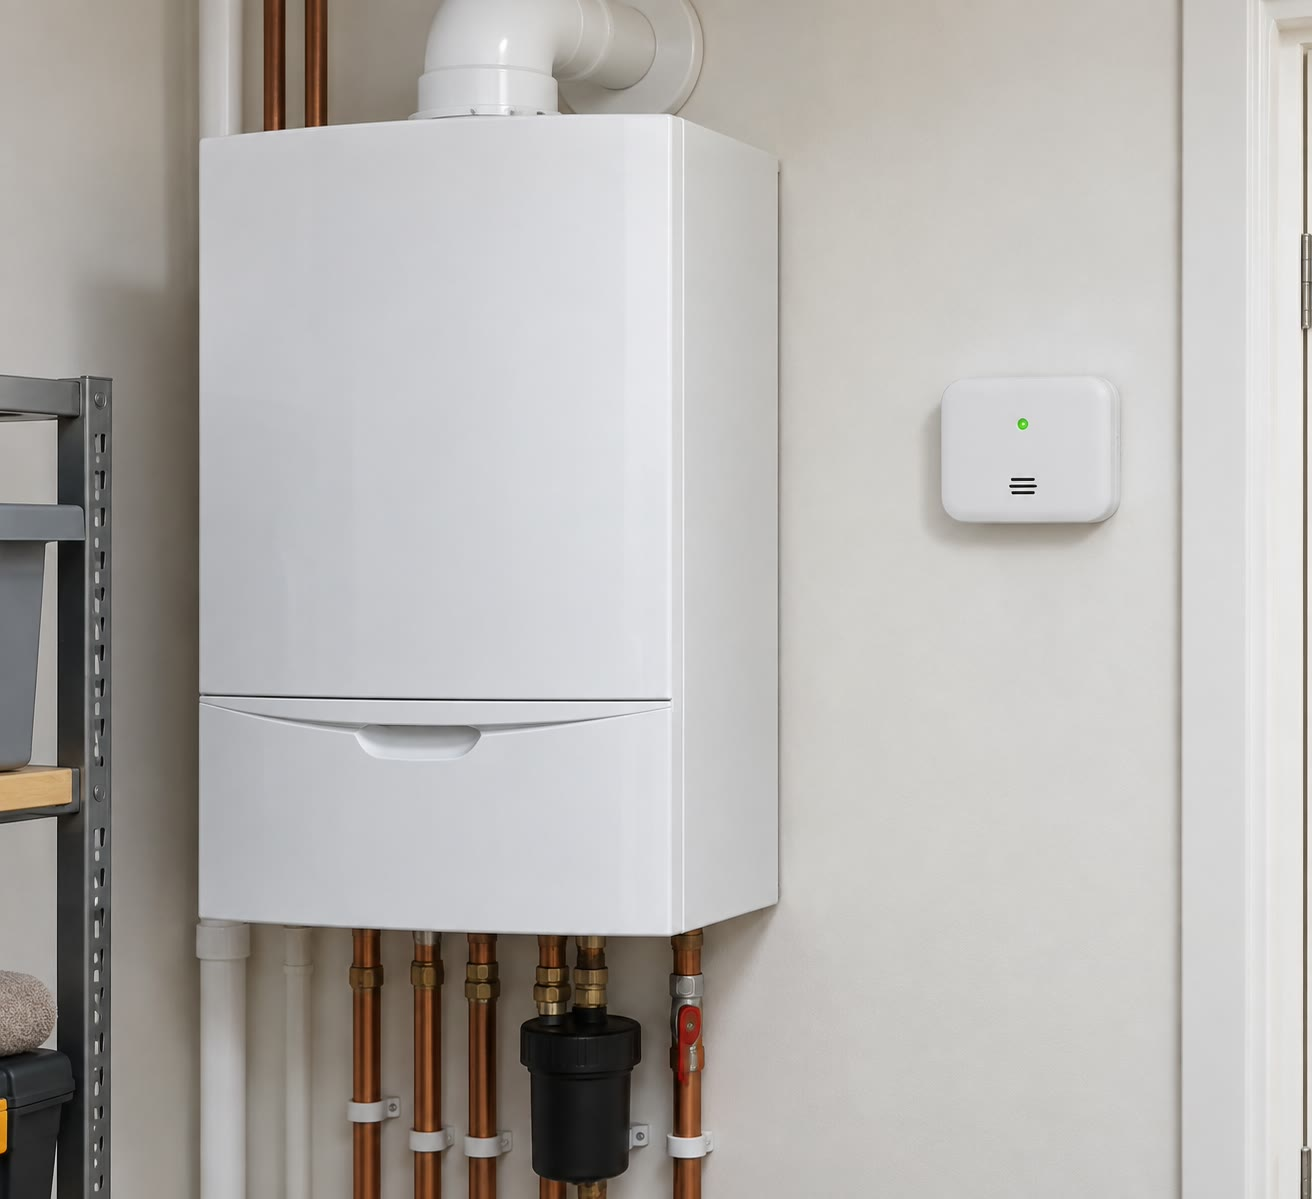
\includegraphics[width=0.45\linewidth]{images/book1/ai/g8-boiler-alarm.jpg}

{\small Une chaudière à gaz et, à côté, un détecteur de monoxyde de
carbone.}
\end{omfigure}

\section{Le dioxyde de carbone et l'effet de serre}

\begin{definition}[Gaz à effet de serre]\label{def:g8:combustion-and-fuels:greenhouse}
Un \emph{gaz à effet de serre}\index{gaz a effet de serre@gaz à effet de serre} est un gaz de
l'\omterm{def:g4:air-a-mixture-of-gases:air}{air} qui laisse passer la lumière du Soleil mais retient une partie de
la chaleur que la surface de la Terre renvoie vers l'espace, et qui
réchauffe ainsi les basses couches de l'atmosphère. La vapeur d'eau, le
dioxyde de carbone et le méthane sont des gaz à effet de serre~; le
diazote et le dioxygène n'en sont pas. (La façon dont cela se produit
est expliquée dans le livre de physique.)
\end{definition}

\begin{proposition}[Le dioxyde de carbone de l'air augmente]\label{prop:g8:combustion-and-fuels:rising}
% ledger: co2:mlo-1959, co2:mlo-2025 (rise 111.4 ppm, +35 %)
La quantité de dioxyde de carbone dans l'\omterm{def:g4:air-a-mixture-of-gases:air}{air} est mesurée sans
interruption depuis 1959 dans un observatoire situé sur une montagne au
milieu de l'océan Pacifique. Elle était de 316 parties par million (ppm)
d'\omterm{def:g4:air-a-mixture-of-gases:air}{air} en 1959 et de 427 ppm en 2025~: une hausse d'environ
\qty{35}{\percent} en une vie humaine, due surtout à la \omterm{def:g4:what-a-fire-needs:burning}{combustion} du
charbon, du pétrole et du gaz naturel. Ce dioxyde de carbone
supplémentaire renforce l'effet de serre et réchauffe le climat.
\end{proposition}

\begin{omfigure}
\begin{tikzpicture}
\begin{axis}[width=0.85\linewidth, height=6cm, xmin=1955, xmax=2030,
    ymin=300, ymax=440, xlabel={année}, ylabel={dioxyde de carbone (ppm)},
    axis lines*=left, ymajorgrids, grid style={gray!20},
    tick label style={font=\small, /pgf/number format/1000 sep={}},
    label style={font=\small}]
\addplot[omDef, thick, mark=*, mark size=0.8pt]
  table[x=year, y=ppm] {figdata/out/grade-8-co2-record.dat};
\node[anchor=west, font=\small] at (axis cs:1962,306) {316 ppm en 1959};
\node[anchor=east, font=\small] at (axis cs:2023,428) {427 ppm en 2025};
\end{axis}
\end{tikzpicture}

{\small Moyenne annuelle du dioxyde de carbone dans l'\omterm{def:g4:air-a-mixture-of-gases:air}{air}, mesurée
depuis 1959 (données du NOAA Global Monitoring Laboratory~; avant 1974,
de la Scripps Institution of Oceanography).}
\end{omfigure}

\section{Combustibles fossiles et combustibles renouvelables}

\begin{definition}[Combustibles fossiles et renouvelables]\label{def:g8:combustion-and-fuels:fossil}
Un \emph{combustible fossile}\index{combustible fossile} --- charbon,
pétrole, gaz naturel --- s'est formé sous terre pendant des millions
d'années à partir des restes de plantes et d'animaux marins anciens. Un
\emph{combustible renouvelable}\index{combustible renouvelable} est
fabriqué à partir de plantes cultivées aujourd'hui, ou de déchets~: le
bois, le biogaz issu du fumier et des déchets alimentaires, l'éthanol
produit à partir de betterave ou de canne à sucre.
\end{definition}

\begin{proposition}[D'où vient le carbone]\label{prop:g8:combustion-and-fuels:cycle}
Les plantes prélèvent du dioxyde de carbone dans l'\omterm{def:g4:air-a-mixture-of-gases:air}{air} pour grandir.
\omterm{def:g4:what-a-fire-needs:burning}{Brûler} un \omterm{def:g8:combustion-and-fuels:fossil}{combustible renouvelable} rend le dioxyde de carbone que ses
plantes avaient pris à l'\omterm{def:g4:air-a-mixture-of-gases:air}{air} quelques années plus tôt. \omterm{def:g4:what-a-fire-needs:burning}{Brûler} un
\omterm{def:g8:combustion-and-fuels:fossil}{combustible fossile} libère du carbone qui était enfermé sous terre
depuis des millions d'années~: cela ajoute du dioxyde de carbone à
l'\omterm{def:g4:air-a-mixture-of-gases:air}{air}.
\end{proposition}

\begin{omfigure}
\begin{tikzpicture}[font=\small,
    box/.style={draw=omDef, fill=omDef!6, rounded corners=2pt, align=center,
      minimum height=0.9cm, text width=2.6cm}]
  \node[box] (air) at (0,3) {dioxyde de carbone\\ dans l'air};
  \node[box] (plants) at (5.6,3) {croissance des\\ plantes (\ce{CO2} pris)};
  \node[box] (fuel) at (5.6,0.4) {bois, biogaz,\\ bioéthanol};
  \node[box, draw=black!50, fill=black!8] (fossil) at (0,0.4) {charbon, pétrole,\\ gaz~: sous terre};
  \draw[->, thick, omProp] (air) -- (plants);
  \draw[->, thick, omProp] (plants) -- (fuel);
  \draw[->, thick, omProp] (fuel) -- (air);
  \node[text=black, font=\footnotesize, align=left, anchor=north west] at (1.5,1.45)
    {combustion,\\ des années après};
  \draw[->, thick, black!60] (fossil) -- node[midway, left, text=black, font=\footnotesize,
    align=right] {combustion~:\\ carbone fossile} (air);
\end{tikzpicture}

{\small Les \omterm{def:g8:combustion-and-fuels:fossil}{combustibles renouvelables} rendent à l'\omterm{def:g4:air-a-mixture-of-gases:air}{air} le carbone que
leurs plantes y avaient pris~; les \omterm{def:g8:combustion-and-fuels:fossil}{combustibles fossiles} ajoutent du
carbone qui était stocké sous terre.}
\end{omfigure}

\begin{omfigure}
\begin{minipage}[t]{0.48\linewidth}\centering
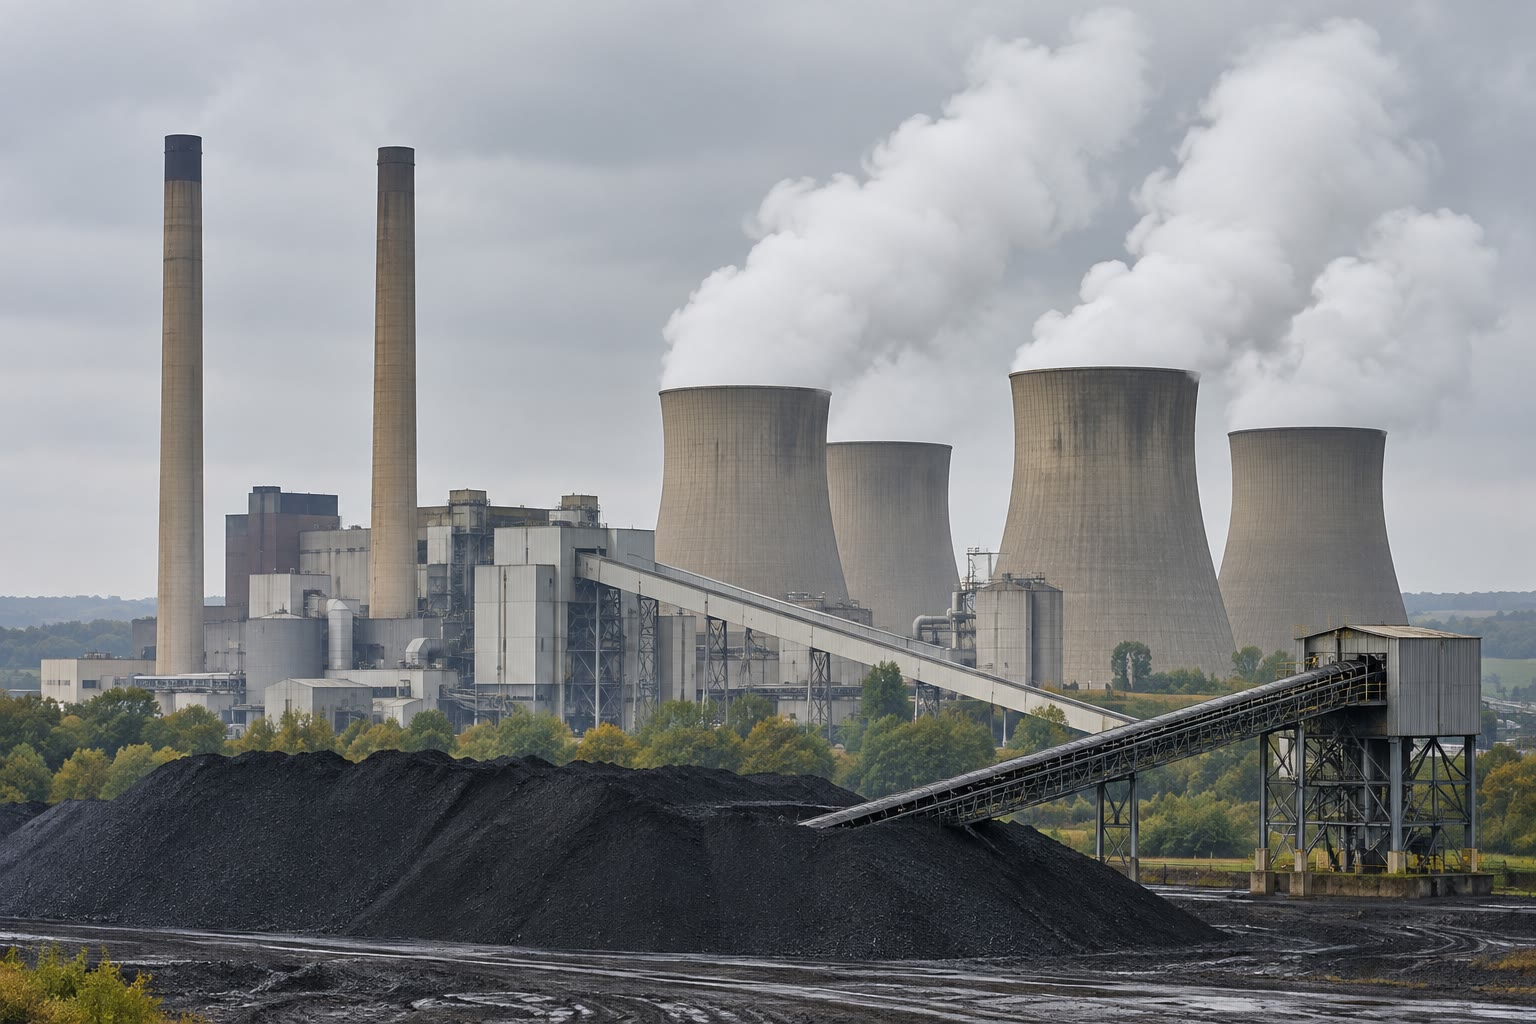
\includegraphics[width=\linewidth,height=4.6cm,keepaspectratio]{images/book1/ai/g8-coal-plant.jpg}

{\small Une centrale électrique au charbon.}
\end{minipage}\hfill
\begin{minipage}[t]{0.48\linewidth}\centering
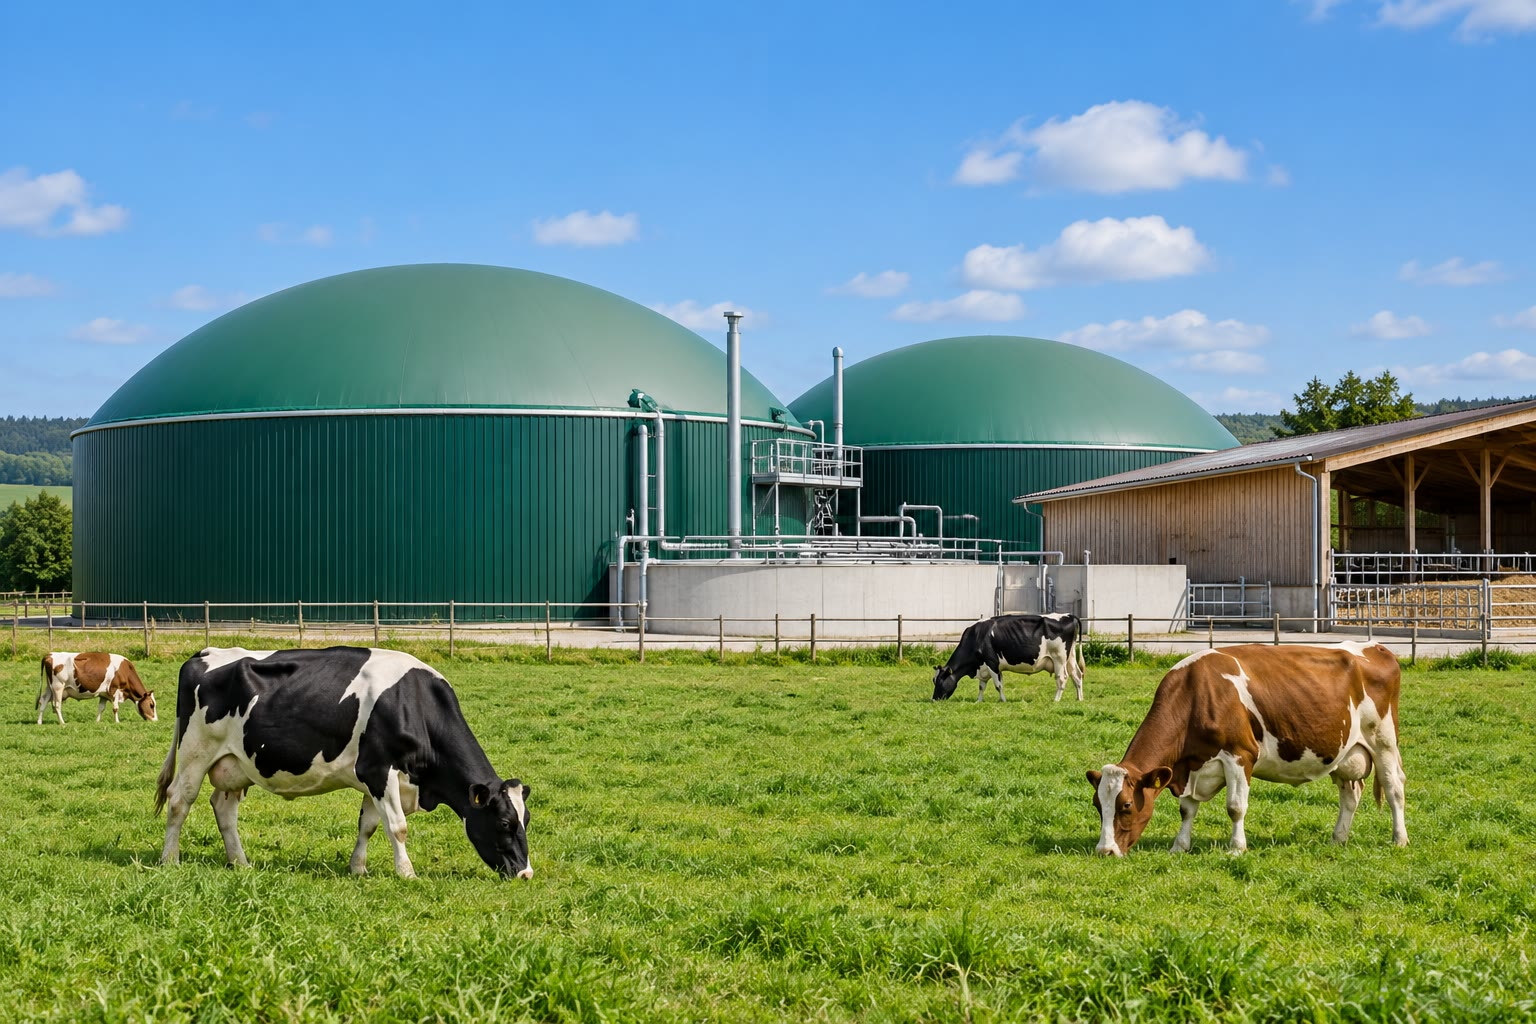
\includegraphics[width=\linewidth,height=4.6cm,keepaspectratio]{images/book1/ai/g8-biogas-farm.jpg}

{\small Une installation de biogaz à la ferme~: le fumier devient un
\omterm{def:g8:combustion-and-fuels:fossil}{combustible renouvelable}.}
\end{minipage}
\end{omfigure}

\section{Exercices}

\begin{exercise}[$\star$]\label{exo:g8:combustion-and-fuels:1}
Écris l'\omterm{def:g8:balanced-equations:equation}{équation ajustée} de la \omterm{def:g8:combustion-and-fuels:complete}{combustion complète} du carbone.
\end{exercise}

\begin{exercise}[$\star$]\label{exo:g8:combustion-and-fuels:2}
Quelle est la différence entre une \omterm{def:g8:combustion-and-fuels:complete}{combustion complète} et une \omterm{def:g8:combustion-and-fuels:complete}{combustion
incomplète}~?
\end{exercise}

\begin{exercise}[$\star$]\label{exo:g8:combustion-and-fuels:3}
Pourquoi dit-on que le monoxyde de carbone est un danger silencieux~?
\end{exercise}

\begin{exercise}[$\star$]\label{exo:g8:combustion-and-fuels:4}
Fossile ou renouvelable~: le charbon, le bois, le gaz naturel, le
biogaz, l'essence, l'éthanol de betterave~?
\end{exercise}

\begin{exercise}[$\star\star$]\label{exo:g8:combustion-and-fuels:5}
Écris l'\omterm{def:g8:balanced-equations:equation}{équation ajustée} de la \omterm{def:g8:combustion-and-fuels:complete}{combustion complète} du propane,
\ce{C3H8}.
\end{exercise}

\begin{exercise}[$\star\star$]\label{exo:g8:combustion-and-fuels:6}
L'éthanol, \ce{C2H6O}, \omterm{def:g4:what-a-fire-needs:burning}{brûle} complètement dans le dioxygène. Ajuste
\ce{C2H6O + O2 -> CO2 + H2O}. % ce-unbalanced-ok (to balance)
\end{exercise}

\begin{exercise}[$\star\star$]\label{exo:g8:combustion-and-fuels:7}
Une casserole tenue au-dessus d'une flamme jaune noircit par-dessous.
Quelle est la substance noire~? Que nous apprend-elle sur la
\omterm{def:g4:what-a-fire-needs:burning}{combustion}~?
\end{exercise}

\begin{exercise}[$\star\star$]\label{exo:g8:combustion-and-fuels:8}
Lis la courbe du dioxyde de carbone~: environ combien de dioxyde de
carbone l'\omterm{def:g4:air-a-mixture-of-gases:air}{air} contenait-il en 1980 et en 2000~? De combien de ppm
a-t-il augmenté en ces vingt ans~?
\end{exercise}

\begin{exercise}[$\star\star$]\label{exo:g8:combustion-and-fuels:9}
Pourquoi \omterm{def:g4:what-a-fire-needs:burning}{brûler} du bois ajoute-t-il moins de dioxyde de carbone à l'\omterm{def:g4:air-a-mixture-of-gases:air}{air},
au fil des années, que \omterm{def:g4:what-a-fire-needs:burning}{brûler} du charbon, bien que les deux donnent du
dioxyde de carbone~?
\end{exercise}

\begin{exercise}[$\star\star$]\label{exo:g8:combustion-and-fuels:10}
Ajuste la \omterm{def:g8:combustion-and-fuels:complete}{combustion incomplète} du carbone en monoxyde de carbone,
\ce{C + O2 -> CO}. % ce-unbalanced-ok (to balance)
\end{exercise}

\begin{exercise}[$\star\star\star$]\label{exo:g8:combustion-and-fuels:11}
De 1959 (316 ppm) à 2025 (427 ppm), de quel pourcentage le dioxyde de
carbone de l'\omterm{def:g4:air-a-mixture-of-gases:air}{air} a-t-il augmenté~? Arrondis à l'unité.
\end{exercise}

\begin{exercise}[$\star\star\star$]\label{exo:g8:combustion-and-fuels:12}
Un chauffage d'appoint au gaz est utilisé dans une petite pièce, fenêtre
fermée. Explique, à l'aide de deux équations de ce chapitre, comment la
\omterm{def:g4:what-a-fire-needs:burning}{combustion} peut passer de complète à incomplète au fil du temps, et
pourquoi c'est dangereux.
\end{exercise}

\section{Problème~: le réchaud sous la tente}

\begin{problem}[{Problème du week-end --- un réchaud de camping, le gaz
qu'il brûle, ce qu'il produit, et pourquoi il n'entre jamais sous une
tente}]
\label{pb:g8:combustion-and-fuels:1}
% ledger: ghs:propane
Un réchaud de camping \omterm{def:g4:what-a-fire-needs:burning}{brûle} du propane, \ce{C3H8}, contenu dans une
cartouche de \qty{450}{g}. En plein \omterm{def:g4:air-a-mixture-of-gases:air}{air}, la flamme est bleue. On prendra
ces proportions en masse, établies à partir de l'\omterm{def:g8:balanced-equations:equation}{équation ajustée}~:
\qty{44}{g} de propane qui brûlent complètement donnent \qty{132}{g} de
dioxyde de carbone.

\medskip
\noindent\textbf{Partie I --- Les équations.}
\begin{enumerate}
  \item Écris l'\omterm{def:g8:balanced-equations:equation}{équation ajustée} de la \omterm{def:g8:combustion-and-fuels:complete}{combustion complète} du propane.
  \item Vérifie-la en comptant les \omterm{def:g7:atoms-and-molecules:atom}{atomes} de chaque sorte de chaque côté.
  \item Ajuste la \omterm{def:g8:combustion-and-fuels:complete}{combustion incomplète}
        \ce{C3H8 + O2 -> CO + H2O}. % ce-unbalanced-ok (to balance)
  \item Laquelle des deux demande le plus de dioxygène par \omterm{def:g7:atoms-and-molecules:molecule}{molécule} de
        propane~?
\end{enumerate}

\medskip
\noindent\textbf{Partie II --- Sous une tente.}
\begin{enumerate}[resume]
  \item Un réchaud allumé dans une tente fermée \omterm{def:g4:what-a-fire-needs:burning}{brûle} bientôt avec une
        flamme jaune. Explique pourquoi.
  \item Quel gaz dangereux se forme alors~? Donne deux de ses propriétés
        qui le rendent difficile à remarquer.
  \item La cartouche de propane porte deux pictogrammes. Nomme-les et dis
        ce que chacun signifie.
  \item Donne deux règles pour utiliser un réchaud de camping en
        sécurité.
\end{enumerate}

\medskip
\noindent\textbf{Partie III --- Le dioxyde de carbone d'une cartouche.}
\begin{enumerate}[resume]
  \item Combien de fois le dioxyde de carbone formé est-il plus lourd que
        le propane brûlé~?
  \item D'où viennent les grammes supplémentaires~?
  \item Le propane est-il un \omterm{def:g8:combustion-and-fuels:fossil}{combustible fossile} ou un \omterm{def:g8:combustion-and-fuels:fossil}{combustible
        renouvelable}~? Le \omterm{def:g4:what-a-fire-needs:burning}{brûler} ajoute-t-il du dioxyde de carbone à
        l'\omterm{def:g4:air-a-mixture-of-gases:air}{air}~?
  \item Calcule la masse de dioxyde de carbone libérée quand une
        cartouche entière de \qty{450}{g} \omterm{def:g4:what-a-fire-needs:burning}{brûle} complètement.
\end{enumerate}
\end{problem}
